% !TEX root = ../../thesis.tex

\section{Electronic architecture} % (fold)
\label{sec:poppy-electronic}

To keep in the spirit of the project as described by its guidelines (see chapter~\ref{cha:methodology}), the electronic architecture has to be simple, easily reproducible, relatively low-cost and modular. Of course the performance of each component is very important and should be correctly dimensioned.

The first version of Poppy (beta) had a handmade electronics architecture, which required hacking several components before soldering them together. This design was not compliant with the design guidelines of Poppy (i.e. easy to use and to reproduce) and was actually the main reason Poppy was considered as a beta version. Recent work has been done toward the simplification and the reproducibility of the electronics part.

Yet the electronic integration is challenging. Indeed, because Poppy has 5 degrees of freedom in the torso, there is not enough room for all electronic components needed. Therefore we had to embed most of them in the head which raises not only a problem of space but also of mass.

Poppy's electronic architecture is based on several key-components communicating with each other (see Figure Ref):
\begin{itemize}
    \item an IO board controlling all the sensorimotor space,
    \item an embedded computing module to permit wireless communication,
    \item a head screen to display emotions or information,
    \item an alimentation board to provide the 12V needed for the motors and 5V needed for electronic systems,
\end{itemize}

\begin{figure}[tb]
    \begin{center}
        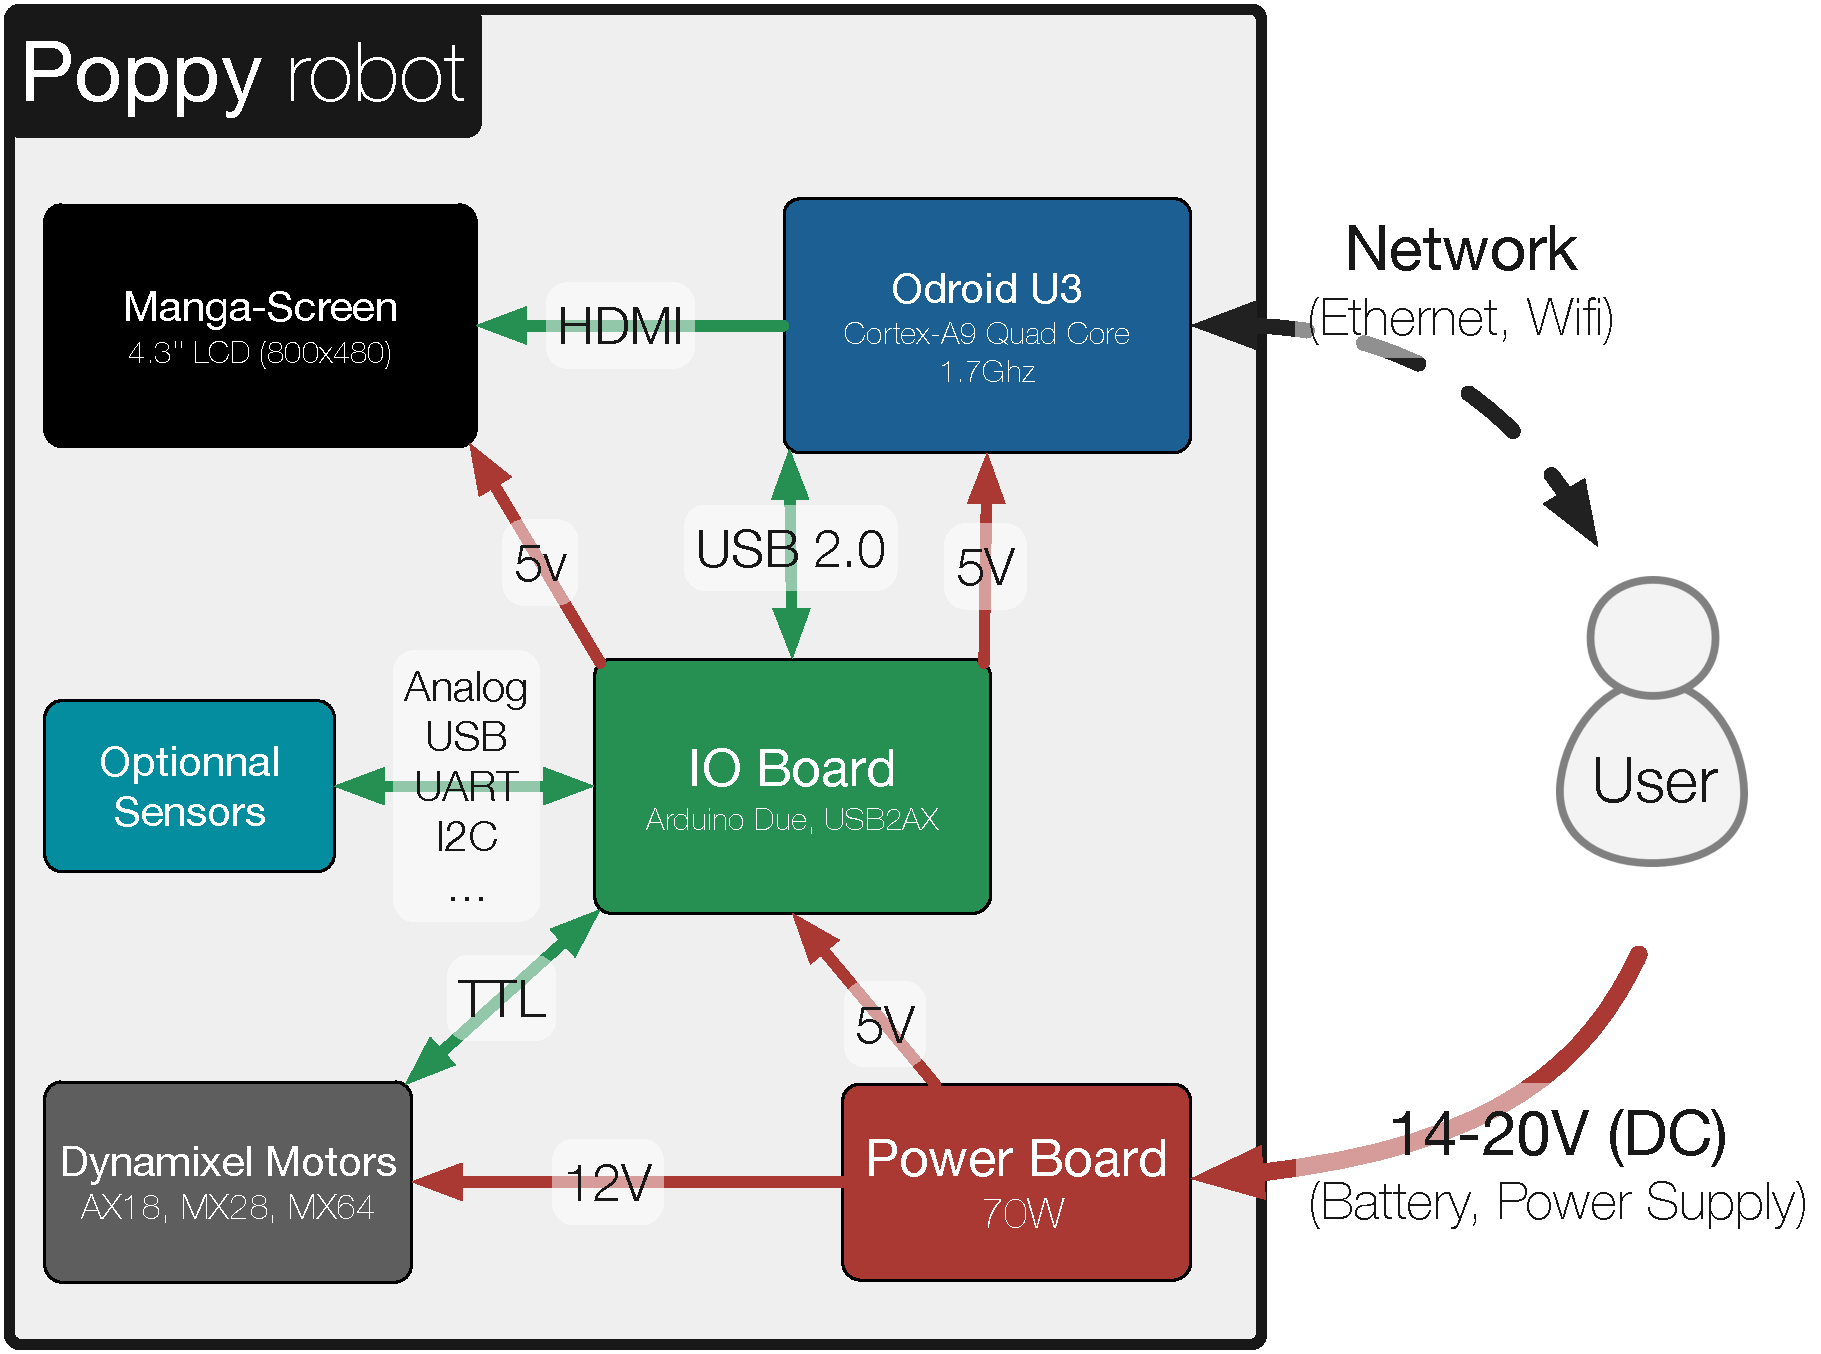
\includegraphics[width=\linewidth]{poppy_electro_archi_overview.pdf}
    \end{center}
    \caption{}

\end{figure}

We will describe in this section, the design choices we made for these various components.

\subsection{Poppy IO Board} % (fold)

With the aim of offering easy-to-use modular electronics architecture and to make it fit in the head of Poppy, we decided to create a custom board\footnote{This board has been developped by Fabien Depraetre during his mster internship}. We could argue it makes the diffusion of the platform more complex, since a custom board is too complex to make by hand and therefore may necessitate the kind of industrialization process we have been trying to avoid since the early days of the project. Nevertheless the maker’s revolution brings novel solutions for producing electronics. Indeed, there are now companies (such as CircuitHub\footnote{\url{https://circuithub.com}}), which offer scalable solution tools from 1 sample to a 10,000 batch. It is possible to upload our design and anyone can ask to have it produced. Of course ordering one part is more expansive but remains relatively low compared to the cost of the robot.

The board we designed included the basic elements needed both for the control of the robot and for its extensibility.


\subsubsection{Motor control} % (fold)
Robotis Dynamixel are normally controlled by the \emph{USB2Dynamixel} but we decided to replace it with USB2AX devices (see \figurename~\ref{fig:usb2ax}). The USB2AX is a small interface to control Dynamixel servomotors from a computer and was designed by Nicolas Saugnier. It plugs into a USB port and has a 3-pin molex connector compatible with the robotis ones.

For use on Poppy, these devices have several main advantages:
\begin{enumerate}
    \item They are a lot smaller than the standard USB2Dynamixel module (16x36mm instead of 35x90mm) (see \figurename~\ref{fig:USB2AX_vs_USB2Dxl}).
    \item They can endure a short-circuit between the DATA and power-supply wire.
    \item They have the sync\_read instruction to read a lot of information very fast, which is not a standard Dynamixel instruction. The USB2AX converts SYNC\_READ into multiple separate READ commands to get data from each servo, then sends back to the computer a single big packet containing all the data. This significantly decreases the effect of USB latency. A SYNC\_READ command reads the same registers in each servo (see \figurename~\ref{fig:usb2ax-perf}).
    \item It is open source so we can extend or adapt this solution to our needs.
\end{enumerate}

\begin{figure}[tb]
\centering
    \subfloat[][]{\label{fig:usb2ax_dongle}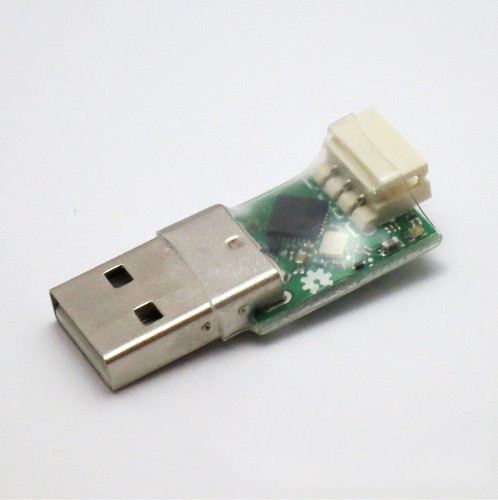
\includegraphics[height=4.5cm]{usb2ax.jpg}}
    \hfil
    \subfloat[][]{\label{fig:USB2AX_vs_USB2Dxl}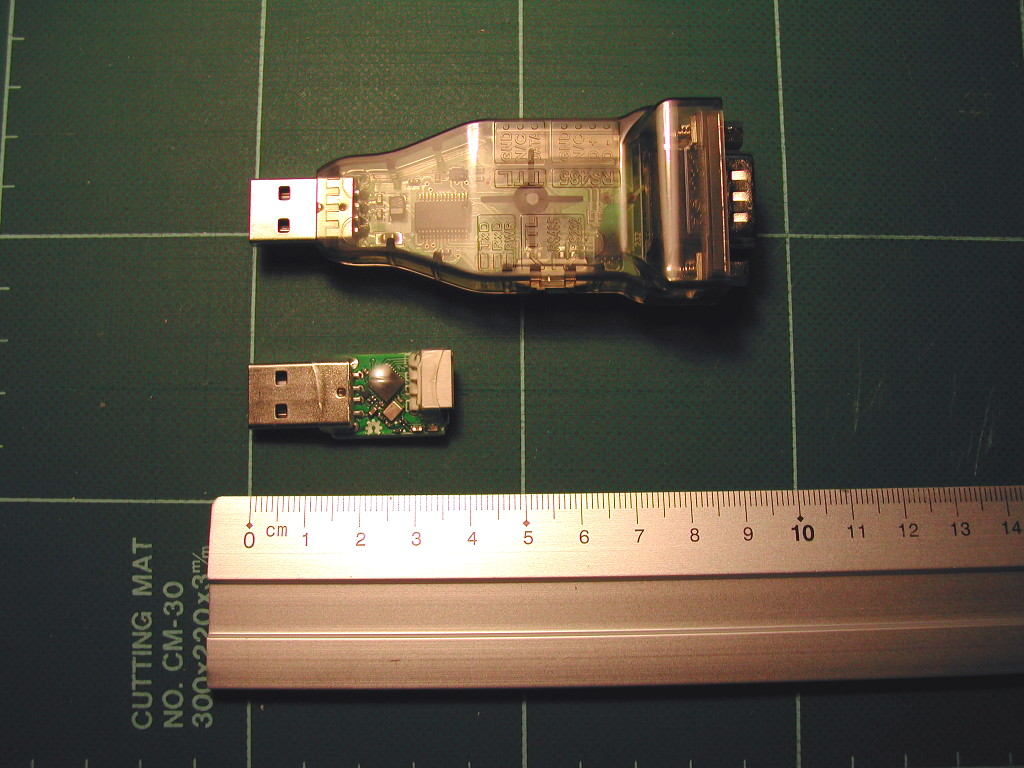
\includegraphics[height=4.5cm]{USB2AX_vs_USB2Dxl.jpg}}\\

    \subfloat[][]{\label{ig:usb2ax-perf}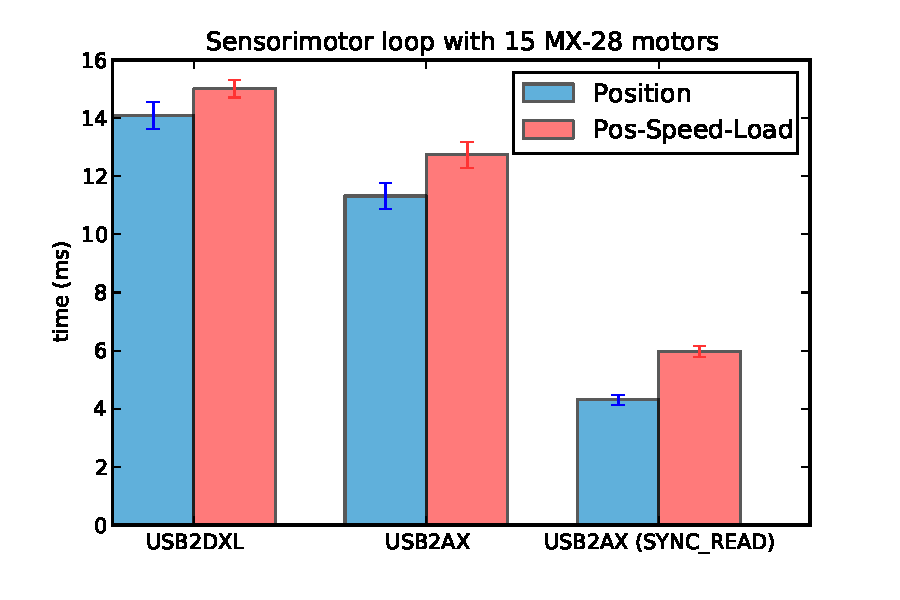
\includegraphics[height=5.5cm]{motor-bench.pdf}}
    \caption{}
    \label{fig:usb2ax}
\end{figure}

This project has always been used on Poppy and greatly helped us to have an effective robot while keeping the space for electronics low.
Because the project is open hardware, we have reused it and embedded it directly on a custom board so that we can make it even smaller by avoiding USB connectors.

\subsubsection{Arduino integration} % (fold)
As we explain in the section REF, the modularity of Poppy’s electronics is achieved thanks to the use of the Arduino environment. For the Arduino integration we decided to use the new Arduino Due based on the Atmel SAM3X8E ARM Cortex-M3 CPU. These board embeds both a powerful microcontroller (84 MHz 32-bit ARM core) and a large number of inputs/outputs: 54 digital input/output pins (of which 12 can be used as PWM outputs), 12 analog inputs, 4 UARTs (hardware serial ports).


\subsubsection{Actual design of the IO Board} % (fold)
The IO board is an open hardware project aiming to simplify the use of Poppy for non-electronic-expert users. Therefore it integrates into one board all components it would be necessary to plug or solder.


This board is based on other open hardware projects previously presented and contains two usb2ax for communication with Robotis actuators, an Arduino Due to permit the extension of the sensors space plus convenient ports to easily plug external devices in. See \figurename~\ref{tab:io-board-specs} for complete details on all the available IO ports.

In addition, it integrates two sensors: an ADXL345 accelerometer, which has four measurement ranges (2g/4g/8g/16g) with up to 13-bit resolution and a data rate of up to 3200Hz; and a ITG-3200 gyroscope, which has a full scale range of +/- 2000\textsuperscript{o}/s with 16-bit resolution and data rate of up to 36kHz.


The board has been designed using KiCad\footnote{Open source EDA software}, the source files are distributed under open source license\footnote{Creative Commons CC-BY-SA} and available on our GitHub project\footnote{\url{https://github.com/poppy-project/poppy-electronics/tree/master/CarteIo}}. The production of the board can be done using CircuitHub\footnote{\url{https://circuithub.com/projects/Poppy_project/CarteIo}} and costs \$250 for one board or \$90 for ten\footnote{The cost decrease with quantity is up to \$50.}.

\begin{figure}[p]
\centering
    \subfloat[][]{\includegraphics[width=\linewidth]{IO_Board.pdf}}


    \subfloat[][]{\label{tab:io-board-specs}
        \begin{tabularx}{0.8\linewidth}{r X}
        \textbf{2x} & high-speed motors buses\\
        \textbf{2x} & UART ports\\
        \textbf{1x} & I2C bus\\
        \textbf{2x} & external USB Ports\\
        \textbf{1x} & accelerometer\\
        \textbf{1x} & gyroscope\\
        \textbf{12x} & anlog pins\\
        \textbf{12x} & digital pins allowing PWM control\\
        \textbf{4x} & 5v ports to supply power to external devices\\
        \end{tabularx}
        }
    \caption{}
    \label{fig:IO-board}
\end{figure}


\subsection{Embedded computing module} % (fold)

The integration of a computing module is rather complex and not fundamental if the robot cannot walk for more than 5 m, therefore the Poppy beta version was controlled using an external computer connected by USB.
However, Poppy is aimed at becoming a shared research platform with people addressing challenges in which embedded control could be necessary. Also as all users have different computer configurations (Windows, MacOS and wide Linux distribution), it is easier to maintain the control software if only one OS is used. Embedding linux allows us to have the control and ensure same performance for every Poppy.

Yet as I said previously, embedding control is complex. Indeed, the computer has to be small enough to fit inside the robot. With such a size, where are mostly ARM based computer. Most works are developed on x86 or 64 architecture and the switch to ARM architecture is not direct. Some software modules used do not exist or are not optimized, leading to major performance problems.

It is the case with one of the most famous micro-computer, the raspberry pi. The first trials we did with Pypot were really disappointing on the performance level. As we can see in section REF, it takes about 10-12 minutes just to read and write a motor position (mostly computing) while it is only 2 minutes on a normal computer (mostly serial communication). Therefore we oriented our choice toward the Hardkernel Odroid U3 board (8\~12 times faster than the Raspberry Pi).

\begin{figure}[p]
    \centering
    \subfloat[][]{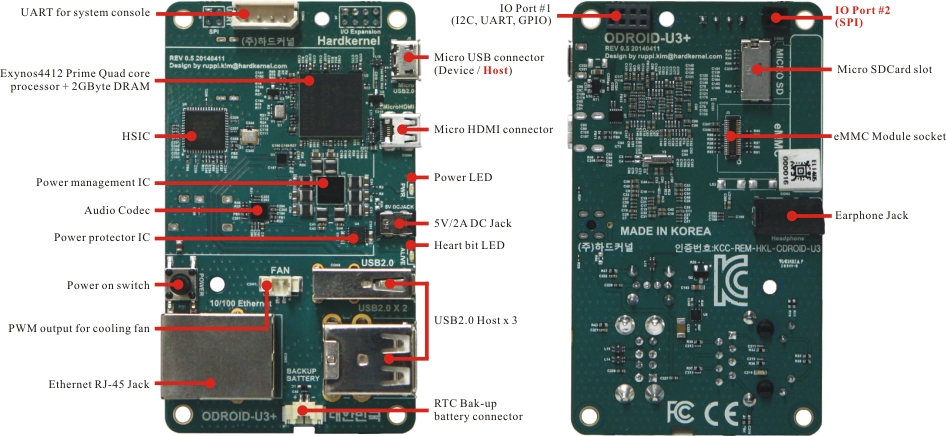
\includegraphics[width=\linewidth]{Odroid_U3.jpg}}


    \subfloat[][]{\begin{tabularx}{\linewidth}{r X}
        % \hline
        \textbf{Processor} & Samsung Exynos4412 Prime Cortex-A9 Quad Core 1.7Ghz with 1MB L2 cache\\
        \textbf{Memory} & 2048MB(2GB) LP-DDR2 880Mega data rate\\
        \textbf{3D Accelerator} & Mali-400 Quad Core 440MHz\\
        \textbf{Video} & supports 1080p via HDMI cable(H.264+AAC based MP4 container format)\\
        \textbf{Video Out} & micro HDMI connector\\
        \textbf{Audio} & Standard 3.5mm headphone jack HDMI Digital\\
        \textbf{LAN} & 10/100Mbps Ethernet with RJ-45 Jack ( Auto-MDIX support)\\
        \textbf{USB2.0 Host} & High speed standard A type connector x 3 ports\\
        \textbf{USB2.0 Device} & ADB/Mass storage(Micro USB), Host mode is possible if the PCB Rev is 0.5 or higher.\\
        \textbf{Display} & HDMI monitor\\
        \textbf{IO Port} & GPIO, UART, I2C, SPI(Board Revision 0.5 or higher)\\
        \textbf{Storage (Option)} & MicroSD Card Slot eMMC module socket\\
        \textbf{Power (Option)} & 5V 2A Power\\
        \textbf{System Software} & Linux : Xubuntu 13.10 or latest version Android : u-boot 2010.12, Kernel 3.0.x, Android 4.x  Full source code is available now.\\
        \textbf{PCB Size} & 83 x 48 mm\\
        \textbf{Weight} & 48g including the heat sink\\
         & \\
        % \hline
        \end{tabularx}
        }
    \caption{Hardkernel Odroid U3 computer board}
    \label{fig:odroid_U3}
\end{figure}

The Hardkernel Odroid U3 (see \figurename~\ref{fig:odroid_U3}) is a low-cost (\$65) and powerful Linux computer embedding a 1.7GHz Quad-Core processor and 2GByte RAM while being very small (83 x 48 mm) and lightweight (48 grams) (see Tab.~\ref{tab:table_feet} for the detail of all specifications).


Among the plug-n-play small computers, the Odroid U3 is currently the most suitable board for our application with regards the size, the computing power and the I/O positions.
Yet as we will explain in the limitations part (see section~\ref{sub:electronic-limitations}), this solution is still not perfectly satisfactory and the use of plug-n-play computers raises a lot of integration problems.

\subsection{Display} % (fold)

The video out port on all new mini computer boards such as Raspberry Pi, Beagle board or Odroid boards is an HDMI port. Finding a small screen (< 7inch) compatible with an HDMI input is really hard and currently only one project exists. The manga-screen (see \figurename~\ref{fig:manga-screen}) is an open source (CC-BY-SA\footnote{see REF}) multi-purpose, HDMI-compatible LCD screen. This board is developed by Elias Bakken and works with a 4.3 inch screen (480x800px) made by Sharp\footnote{Sharp LQ043Y1DX07}.

\begin{figure}[ht]
\centering
    \subfloat[][]{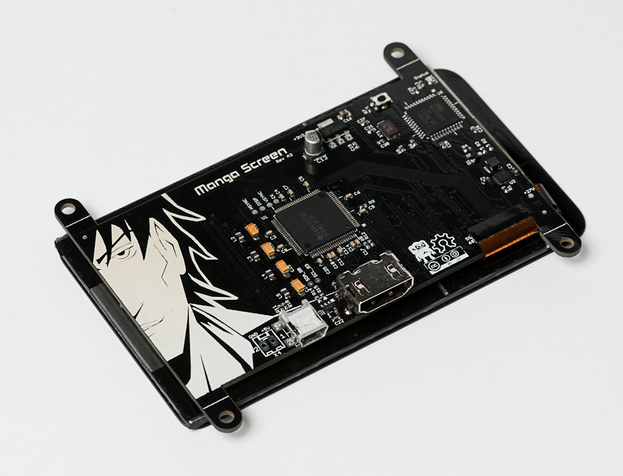
\includegraphics[height=4.9cm]{manga-screen.png}}
    \hfil
    \subfloat[][]{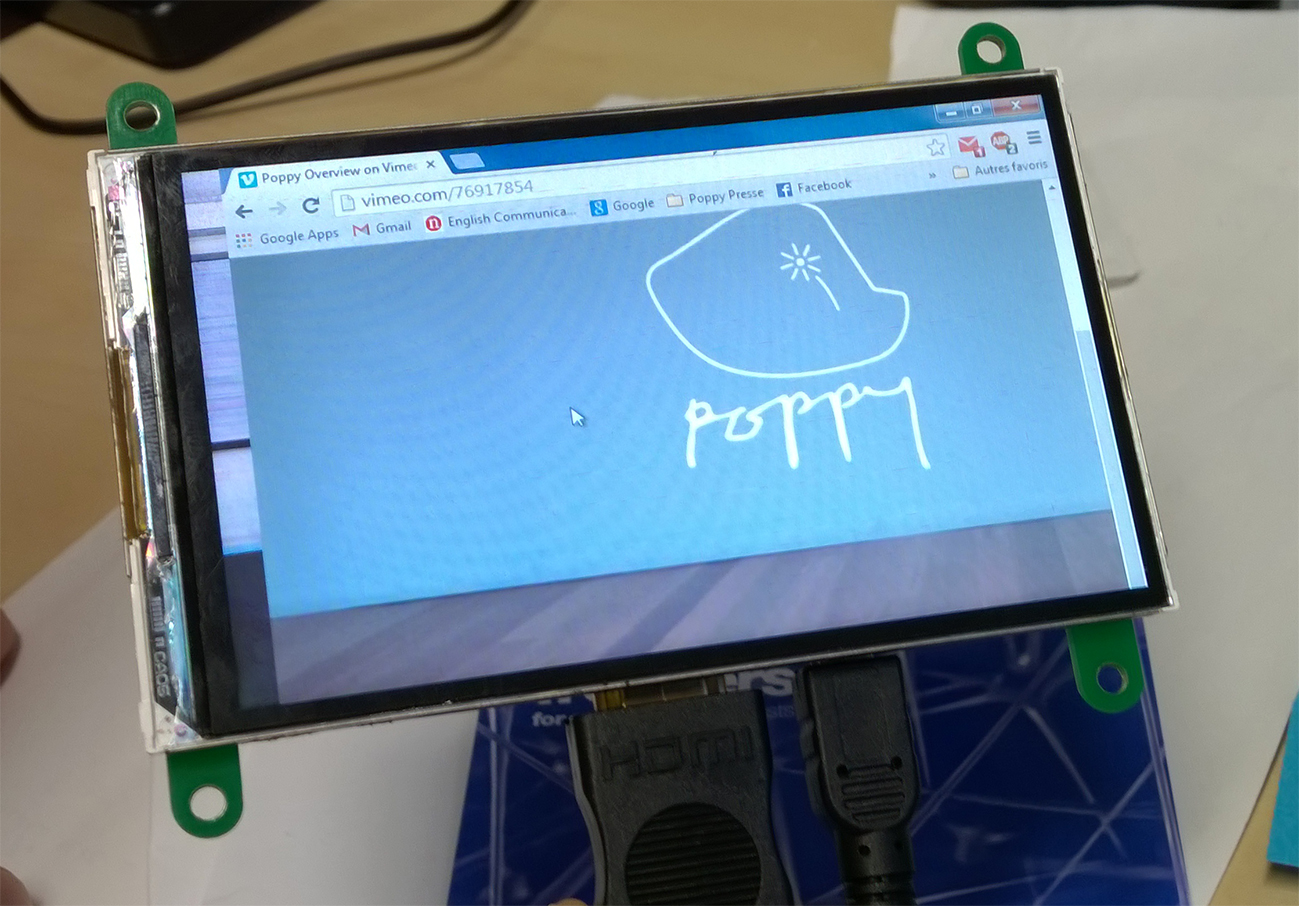
\includegraphics[height=4.9cm]{poppy_screen.jpg}}
    \caption{}
    \label{fig:manga-screen}
\end{figure}

The integration of a LED matrix panel would be easier but it would require creating drivers for the display.
Using a HDMI display connected to a Linux computer allows users to easily display information or animation on the screen as if it were on their monitor. Therefore users are free to use any tools they like such as Processing, OpenGL, VLC or whatever. This flexibility would not be possible with a matrix LED panel which would have required controlling the information displayed with Arduino programming.

\subsection{Power Supply} % (fold)
\label{ssub:alimentation}

\subsubsection{Power board} % (fold)
Power for the current Poppy is supplied by Robotis. This solution is really low-cost in the tens of euros range but it is limited. Indeed, the Robotis power supply provides directly 12V@5A dans is plugged directly into the robot. Yet the wire is short and not really convenient. It would be a better solution to have on board active components allowing the conversion of a wide range of power supplies to the one needed for Poppy. In particular, we could be compatible with a standard laptop power supply (18-22V).

This work is still in progress and the chosen solution will be presented in the final version of this thesis.


\subsubsection{The battery issue} % (fold)

One issue associated with the batteries is the mass. Indeed 3.6V battery cell weights around 45 grams and we need at least 4 cells to supply the 12V needed for Poppy, thus a 14,4V pack weights almost 200 grams (see \figurename~\ref{fig:battery_specs}). For comparison a MX-28 Dynamixels weights 72grams so a battery pack suitable for Poppy weighs approximately the same mass as 3 motors.
In addition, the overall size is quite big with 18mm x 65mm x 18mm (see \figurename~\ref{fig:battery_size}) and makes the integration complicated in a multi-articulated and small robot like Poppy.

Poppy is not yet able to walk by itself, being energetically autonomous does not seem a high priority. Thus we chose to not include batteries in Poppy’s current electronic architecture. Yet, we hope the community will try to address this challenge and maybe find original and suitable solutions.

\begin{figure}[tb]
\centering
    \subfloat[][]{\label{fig:battery_size}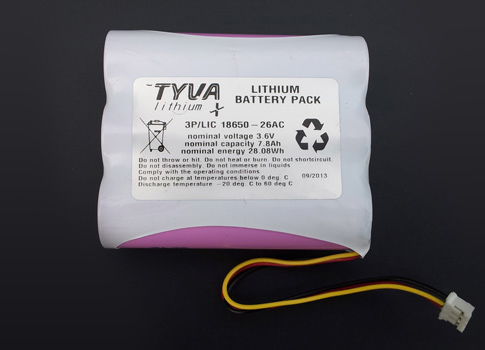
\includegraphics[height=3.5cm]{tyva_battery_pack.jpg}}
    \hfil
    \subfloat[][]{\label{fig:battery_specs}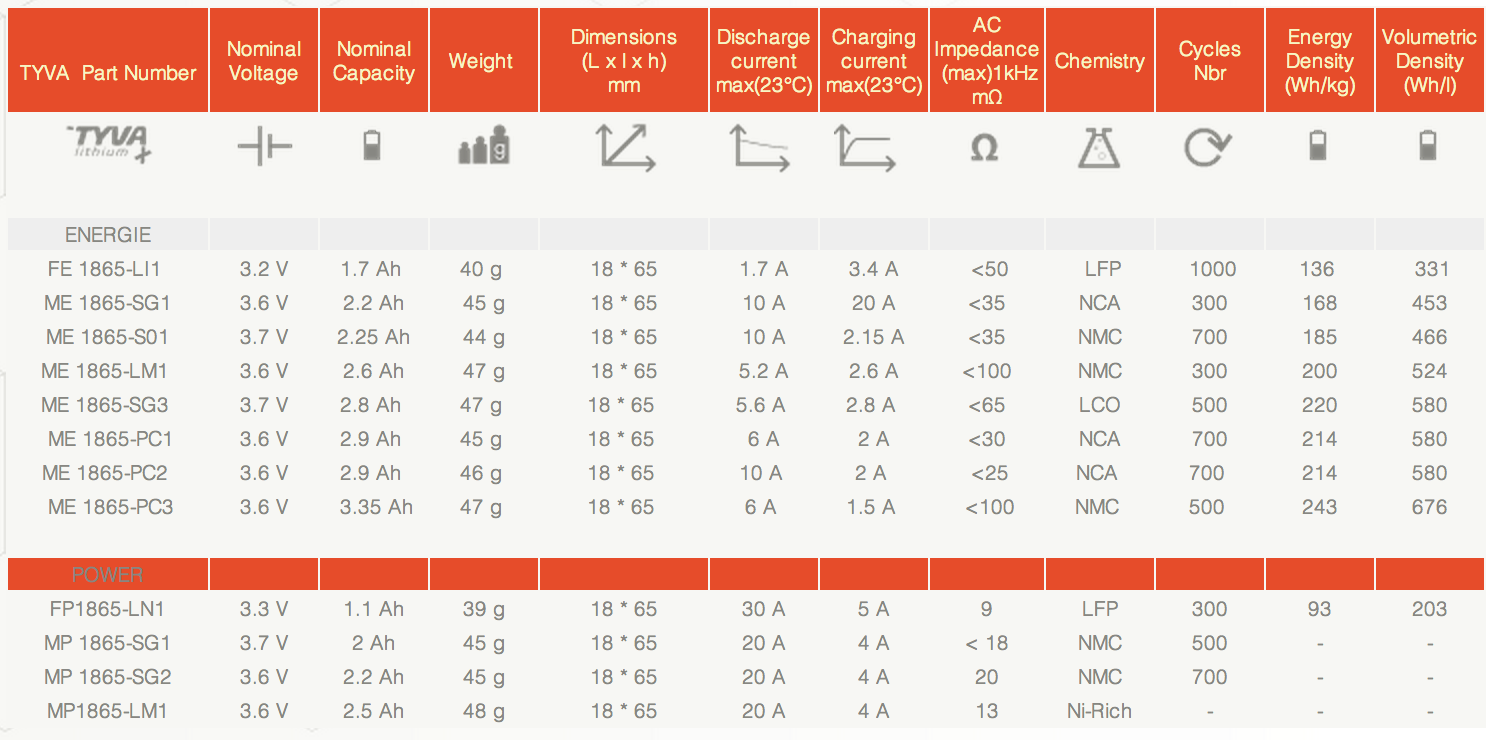
\includegraphics[height=4cm]{tyva_batteries.png}}\\
    \caption{}
    \label{fig:tyva_batteries}
\end{figure}

However, using Poppy away from any power source is still possible. Is it indeed rather simple to connect external 12V batteries. These batteries can be easily found on the internet and have already been tested with Poppy for an artistic project where Poppy had to be surrounded by nature\footnote{see associated projects on our forum}.

